\begin{problem}{Gyakkyou Burai Kaiji}
{gyakkyou.in}{gyakkyou.out}
{4 seconds}{256 mebibytes}

% Author: Akai

\epigraph
{
You shouldn't let kings like myself draw twice.
}{}

Once before he was there.
Kaiji lost everything.
The only thing he kept was his miserable life.

%\begin{figure}
%{10.5cm}
%{
    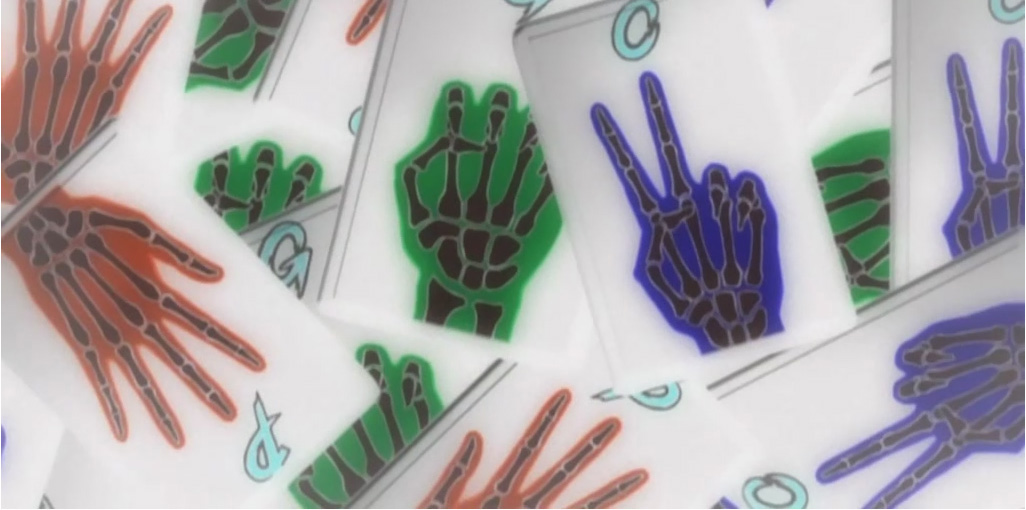
\includegraphics [width=10cm]{pics/g.jpg}
%}
%\end{figure}

The rules of this game are almost the same.
There are $N$ different types of cards.
All types are numbered from $1$ to $N$, inclusive.
Kaiji stores his cards in decks.
He always puts cards of the same type in the same deck,
and cards of different types in different decks.
Index of every deck is equal to the index of type of cards it contains.

At any moment of time, Kaiji can have from $0$ to $999\,999\,999$ cards
of each type.
However, now gamblers cannot buy, sell or exchange cards.
Thus the amount of cards of each type Kaiji has
stays the same during the whole game.
During a turn, Kaiji can gamble using only decks with indices
from segment $[i, j]$ where $i$ and $j$ are the parameters of the turn.

Kaiji has already examined the behavior and strategies of all gamblers
and invented a winning strategy.
All he needs now is to quickly find the answers to the following type
of questions:
on a turn with parameters $i$ and $j$, what is the amount of cards
in the $k$-th largest deck among the decks he can use?
Help him answer these questions.

\InputFile

The first line contains an integer $N$, the amount of types of cards
($1 \leq N \leq 450\,000$). 

The second line is used to generate integers $a_i$, the initial amount
of cards of each type which Kaiji has ($0 \leq a_i < 10^9$).
It contains three integers $a_1$, $l$ and $m$
($0 \leq a_1, l, m < 10^9$); for $2 \leq i \leq N$,
$$a_i = (a_{i-1} \cdot l + m) \bmod 10^9\text{.}$$

The third line contains an integer $B$,
the number of opponents ($1 \leq B \leq 1000$).
$B$ lines follow, each describing the set of games with a particular opponent.
Each set is described by ten integers.
The first one is $G$, the number of games played with that opponent.
Then follow $x_1$, $l_x$ and $m_x$, then $y_1$, $l_y$ and $m_y$,
and finally, $k_1$, $l_k$ and $m_k$
($1 \leq x_1 \leq y_1 \leq N$, $1 \leq k_1 \leq y_1 - x_1 + 1$,
$0 \leq l_x, m_x, l_y, m_y, l_k, m_k < 10^9$).
These are used to generate auxiliary sequences $x_g$ and $y_g$ and
the actual parameters $i_g$, $j_g$ and $k_g$ for $1 \leq g \leq G$:
$$
\begin{array}{ccll}
x_g & = & ((i_{g - 1} - 1) \cdot l_x + m_x) \bmod N) + 1, & 2 \leq g \leq G \\
y_g & = & ((j_{g - 1} - 1) \cdot l_y + m_y) \bmod N) + 1, & 2 \leq g \leq G \\
i_g & = & \min(x_g, y_g), & 1 \leq g \leq G \\
j_g & = & \max(x_g, y_g), & 1 \leq g \leq G \\
k_g & = & (((k_{g - 1} - 1) \cdot l_k + m_k) \bmod (j_g - i_g + 1)) + 1,
& 2 \leq g \leq G \\
\end{array}
$$
The generated parameters mean that in $g$-th game with the current opponent,
Kaiji wants to know the amount of cards in the $k_g$-th largest deck among
his decks with indices from segment $[i_g, j_g]$.

The total number of games played by Kaiji doesn't exceed $600\,000$.

\OutputFile

For each game $g$ with each opponent $b$, find the number of cards in $k_g$-th
biggest deck among his decks with indices from segment $[i_g, j_g]$.
Output one number: the sum of these values.

\Example

\begin{example}
\exmp{
5
1 1 1
5
1 1 0 0 3 0 0 2 0 0
1 2 0 0 5 0 0 3 0 0
1 1 0 0 5 0 0 5 0 0
1 3 0 0 3 0 0 1 0 0
1 1 0 0 4 0 0 1 0 0
}{
15
}%
\end{example}

\medskip

Kaiji has $i$ cards of $i$-th type for all $i = 1, 2, 3, 4, 5$.
Each of these types was chosen exactly once.
So the answer is $15$.

\end{problem}
